\documentclass{beamer}


\DeclareMathOperator*{\argmin}{arg\,min}
\DeclareMathOperator*{\argmax}{arg\,max}


\newcommand{\matrixl}{\left|\left|}
\newcommand{\matrixr}{\right|\right|}

\newcommand{\sign}{\mbox{sign}\,}
\newcommand{\F}{\mathcal{F}}
\newcommand{\Hh}{\mathcal{H}}
\newcommand{\R}{\mathbb{R}}
\newcommand{\E}{\mathbb{E}}
\newcommand{\N}{\mathbb{N}}
\newcommand{\Be}{\mbox{Be}}
\newcommand{\Reg}{\mbox{Regret}}
\newcommand{\dkl}{d_{\mbox{\tiny KL}}}
\newcommand{\Ss}{\mathcal{S}}
\newcommand{\ltwo}{\log_2 }
\newcommand{\A}{\mathcal{A}}

% пустое слово
\def\eps{\varepsilon}

% регулярные языки
\def\eqdef{\overset{\mbox{\tiny def}}{=}}
\newcommand{\niton}{\not\owns}


\usepackage{amsmath}
\usepackage{wrapfig}
\usepackage{enumerate}
\usepackage[makeroom]{cancel}
\usepackage{multicol,multirow}
\usepackage{hyperref}
\usepackage{tabularx}
\usepackage{amsfonts}
\usepackage{amssymb}
\usepackage{amsmath}
\usepackage{amsthm}

\usepackage[utf8]{inputenc}
\usepackage[russian]{babel}
\usepackage{amsmath,mathrsfs,mathtext}
\usepackage{graphicx, epsfig}
\usetheme{Warsaw}%{Singapore}%{Warsaw}%{Warsaw}%{Darmstadt}
\usecolortheme{sidebartab}
\definecolor{beamer@blendedblue}{RGB}{100,30,100}
%----------------------------------------------------------------------------------------------------------
\title[\hbox to 56mm{Обучение с подкреплением  \hfill\insertframenumber\,/\,\inserttotalframenumber}]
{Нижние границы на regret в обучении с подкреплением}
\author[Сергей Володин]{\large \\Сергей Володин}
\institute{\large МФТИ}

\date{}
%-------------------------------------------------------
\begin{document}
%-------------------------------------------------------
\begin{frame}
\titlepage
\end{frame}
%-------------------------------------------------------
\begin{frame}{Обучение с подкреплением}
%Обучение с подкреплением: схема агент-среда, положение в других сферах
Агент взаимодействует со средой:
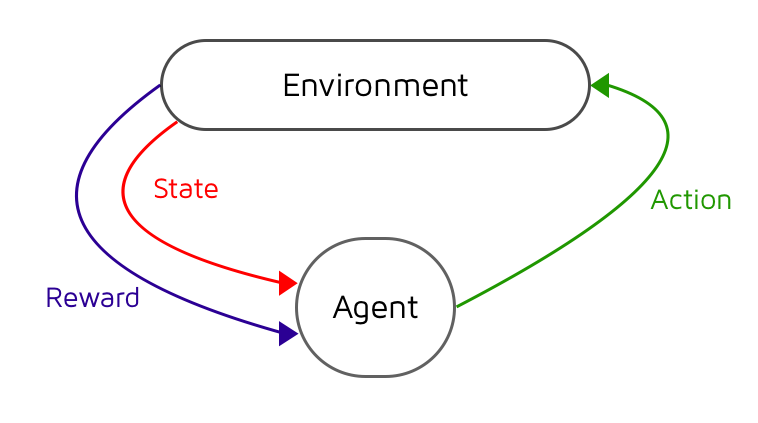
\includegraphics[width=200px]{RL.png}
\end{frame}

\begin{frame}{Определения}
%\theoremstyle{definition}
%\newtheorem{definition}{Определение}[section]
%\newtheorem{lemma}{Лемма}[section]
%\newtheorem{theorem}{Теорема}[section]
\begin{definition}{(Марковский процесс принятия решений)}
	
	ММПР~--- это кортеж $(\mathcal{S}, \mathcal{A}, R, P)$, где
	\begin{enumerate}
		\item $\mathcal{S}=\{1,...,S\}$~--- множество состояний среды
		\item $\mathcal{A}=\{1,...,A\}$~--- множество действий, доступных агенту
		\item $R(s,a)$~--- функция награды. Для данных $s\in \Ss$ и $a\in\A$ случайная величина $R(s, a)\in[0,1]$~--- награда за действие
		\item $P(s,a)$~--- функция переходов. Для данных $s\in \Ss$ и $a\in\A$ случайная величина $P(s, a)\in\Ss$~--- новое состояние среды
	\end{enumerate}
\end{definition}

\begin{definition}{(Взаимодействие агента со средой)}
	
	Имеется ММПР $(\Ss,\A,R,P)$. Вводится время $t\in\N$. Для каждого момента времени \ref{RL}:
	\begin{enumerate}
		\item Агент получает состояние $s_t\in \Ss$
		\item Агент выбирает действие $a_t\in\A$
		\item Агент получает награду $r_t\sim R(s_t,a_t)\in[0,1]$
		\item Среда переходит в новое состояние $s_{t+1}\sim P(s_t,a_t)$
	\end{enumerate}
\end{definition}

\begin{definition}{(Политика)}
	Имеется ММПР $(\Ss,\A,R,P)$.
	
	Политика $\mu$~--- отображение $\mu\colon \Ss\to\A$. То есть, каждому состоянию $s\in\Ss$ сопоставляется действие агента $a\in\A$
\end{definition}

\begin{definition}{(Средняя награда)}
	Имеется ММПР $M=(\Ss, \A,R,P)$, а также политика $\mu$.
	
	$$\lambda_{\mu}^M(s)=\lim\limits_{T\to\infty}\E_{M,\mu}\left[\frac{1}{T}\sum\limits_{t=1}^T\overline{r}(s_t,a_t)\big|s_1=s\right]$$
	
	где $\overline{r}(s,a)=\E R(s,a)$~--- средняя награда в $(s,a)$
	
	То есть, $\lambda_{\mu}^M(s)$~--- средняя награда за бесконечное время при следовании политике $\mu$ в ММПР $M$, если стартовать из состояния $s\in\Ss$. В некотором смысле это <<ценность>> состояния $s$.
	
	Политика $\mu^M$ оптимальна для $M$, если $\mu^M\in\argmax\limits_{\mu}\lambda^M_{\mu}(s)$ для всех $s\in\Ss$. То есть, при старте из любого состояния $s$ политика $\mu$ максимизирует среднюю награду за бесконечное время.
	
	Величина $\lambda_*^M(s)=\lambda_{\mu^M}^M(s)$ называется оптимальной средней наградой.
\end{definition}

\begin{definition}{(История)}
	Имеется ММПР $M=(\Ss,\A,R,P)$. История к моменту времени $t$~--- кортеж $$\Hh_t=(s_1,a_1,r_1,...,s_{t-1},a_{t-1},r_{t-1})$$
	То есть, это последовательный <<журнал>> всех состояний, действий и наград, которые произошли во время взаимодействия агента со средой.
\end{definition}

\begin{definition}{(Алгоритм обучения с подкреплением)}
	Имеется ММПР $M=(\Ss, \A,R,P)$. Алгоритм обучения с подкреплением $\pi$~--- это последовательность функций $\pi=\{\pi_t\big|t\in\N\}$, где $\pi_t$~--- функция, сопоставляющая истории $\Hh_t$ распределение над политиками $\pi_t(\Hh_t)$
	
	То есть, алгоритм $\pi$ получает историю $\Hh_t$ в момент времени $t$ и возвращает распределение над политиками $\pi_t(\Hh_t)$. Далее выполняется сэмплинг $\mu_t\sim\pi_t(\Hh_t)$ из этого распределения, и агент возвращает действие $\mu_t(s_t)$.
	
	Каждое распределение $\pi_t$ должно обладать следующим свойством: если переставить действия и состояния биекциями $s\colon \Ss\to\Ss$ и $a\colon \A\to\A$ в истории $\Hh_t$, получив историю $\Hh_t'$, то распределение над <<исходными>> политиками не изменится, а именно:
	$$(\pi_t(\Hh_t'))(\mu')=(\pi_t(\Hh_t))(a^{-1}\circ\mu'\circ s^{-1})$$
	
	Это свойство означает, что алгоритм действительно получает информацию о среде, а не просто выбирает всегда одно и то же действие.
	
	{\em Данное свойство необходимо для симметрии в Теореме 4.1. В оригинальной статье \cite{lower_bounds} это свойство на самом деле не выполняется, а в более ранней \cite{bubeck} используется другой приём}
\end{definition}

\begin{definition}{(Сожаление)}
	Имеется ММПР $M=(\Ss, \A,R,P)$ и агент $\pi$.
	
	Сожаление агента $\pi$ в момент времени $T$ для начального состояния $s$ в цепи $M$ определяется следующим образом:
	$$\Reg(T,\pi,M,s)=\sum\limits_{t=1}^T(\lambda^M_{\mu^M}(s)-r_t)=T\lambda_*^M(s)-\sum\limits_{t=1}^Tr_t$$
	
	То есть, агент взаимодействует со средой, которая изначально находится в состоянии $s$ в течение $T$ шагов времени. В этом процессе им получаются награды $\{r_i\}_{i=1}^T$.
	
	За всё время $T$ агент мог бы действовать оптимально. Тогда можно ожидать, что он бы получил около $T\lambda_*^M(s)$ награды, так как $\lambda_*^M$~--- средняя награда для состояния $s$. Вместо этого он получил только $\sum\limits_{t=1}^Tr_t$.
	
	Заметим, что $\Reg(T,\pi,M,s)$~--- случайная величина (случайность берётся как из недетерминированности агента, так и из недетерминированности среды)
\end{definition}
\end{frame}

\end{document} 